% Topic 6.1: The Convergence Thesis
% Self-contained Beamer presentation (40 slides)
\documentclass[11pt,aspectratio=169]{beamer}
\usetheme{Madrid}

% ======================= PACKAGES =======================
\usepackage{graphicx}
\usepackage{booktabs}
\usepackage{adjustbox}
\usepackage{multicol}
\usepackage{amsmath}
\usepackage{amssymb}
\usepackage{tikz}
\usetikzlibrary{arrows,shapes,positioning,shadows,trees}
\usepackage{listings}
\usepackage{xcolor}

% ======================= COLOR DEFINITIONS =======================
% Primary color scheme: Blue/Teal for Digital Finance
\definecolor{dfblue}{RGB}{0,102,204}
\definecolor{dfteal}{RGB}{0,153,153}
\definecolor{dfcyan}{RGB}{51,187,204}
\definecolor{dflightblue}{RGB}{153,204,255}
\definecolor{dflightblue2}{RGB}{173,214,255}
\definecolor{dflightblue3}{RGB}{193,224,255}
\definecolor{dflightblue4}{RGB}{213,234,255}

% Accent colors for finance applications
\definecolor{dfgreen}{RGB}{44, 160, 44}
\definecolor{dfred}{RGB}{214, 39, 40}
\definecolor{dforange}{RGB}{255, 127, 14}
\definecolor{dfgray}{RGB}{127, 127, 127}

% Utility colors
\definecolor{lightgray}{RGB}{240, 240, 240}
\definecolor{midgray}{RGB}{180, 180, 180}
\definecolor{codebg}{RGB}{245, 245, 245}

% ======================= THEME CUSTOMIZATION =======================
% Apply Digital Finance color scheme to Madrid theme
\setbeamercolor{palette primary}{bg=dflightblue3,fg=dfblue}
\setbeamercolor{palette secondary}{bg=dflightblue2,fg=dfblue}
\setbeamercolor{palette tertiary}{bg=dfteal,fg=white}
\setbeamercolor{palette quaternary}{bg=dfblue,fg=white}

\setbeamercolor{structure}{fg=dfblue}
\setbeamercolor{section in toc}{fg=dfblue}
\setbeamercolor{subsection in toc}{fg=dfteal}
\setbeamercolor{title}{fg=dfblue}
\setbeamercolor{frametitle}{fg=dfblue,bg=dflightblue3}
\setbeamercolor{block title}{bg=dflightblue2,fg=dfblue}
\setbeamercolor{block body}{bg=dflightblue4,fg=black}

% Remove navigation symbols for cleaner look
\setbeamertemplate{navigation symbols}{}

% Clean itemize/enumerate
\setbeamertemplate{itemize items}[circle]
\setbeamertemplate{enumerate items}[default]

% Margins for readability
\setbeamersize{text margin left=8mm,text margin right=8mm}

% ======================= LISTINGS CONFIGURATION =======================
% Python code style
\lstdefinestyle{pythonstyle}{
    language=Python,
    basicstyle=\ttfamily\footnotesize,
    keywordstyle=\color{dfblue}\bfseries,
    stringstyle=\color{dforange},
    commentstyle=\color{dfgray}\itshape,
    numberstyle=\tiny\color{dfgray},
    numbers=left,
    numbersep=5pt,
    backgroundcolor=\color{codebg},
    showspaces=false,
    showstringspaces=false,
    showtabs=false,
    frame=single,
    rulecolor=\color{midgray},
    tabsize=4,
    captionpos=b,
    breaklines=true,
    breakatwhitespace=false,
    escapeinside={(*@}{@*)},
    xleftmargin=10pt,
    xrightmargin=10pt
}

% Solidity code style
\lstdefinestyle{soliditystyle}{
    language=Java, % closest approximation
    basicstyle=\ttfamily\footnotesize,
    keywordstyle=\color{dfteal}\bfseries,
    stringstyle=\color{dforange},
    commentstyle=\color{dfgray}\itshape,
    numberstyle=\tiny\color{dfgray},
    numbers=left,
    numbersep=5pt,
    backgroundcolor=\color{codebg},
    showspaces=false,
    showstringspaces=false,
    showtabs=false,
    frame=single,
    rulecolor=\color{midgray},
    tabsize=2,
    captionpos=b,
    breaklines=true,
    breakatwhitespace=false,
    escapeinside={(*@}{@*)},
    xleftmargin=10pt,
    xrightmargin=10pt,
    morekeywords={pragma, contract, function, returns, public, private, view, pure, payable, address, uint256, mapping, event, modifier}
}

% Inline code command
\newcommand{\code}[1]{\texttt{\color{dfblue}#1}}

% ======================= CUSTOM COMMANDS =======================
% Bottom annotation (Madrid-style)
\newcommand{\bottomnote}[1]{%
\vfill
\vspace{-2mm}
\textcolor{dflightblue2}{\rule{\textwidth}{0.4pt}}
\vspace{1mm}
\footnotesize
\textbf{#1}
}

% Compact list spacing
\newcommand{\compactlist}{%
\setlength{\itemsep}{0pt}%
\setlength{\parskip}{0pt}%
\setlength{\parsep}{0pt}%
}

% Chart placeholder
\newcommand{\chartplaceholder}[2][5cm]{%
\begin{center}
\begin{adjustbox}{max width=0.95\textwidth, max height=#1}
\framebox[\textwidth][c]{%
\rule{0pt}{#1}%
\textcolor{midgray}{[#2]}%
}
\end{adjustbox}
\end{center}
}

% ======================= FINANCE NOTATION MACROS =======================
% Probability and statistics
\newcommand{\E}{\mathbb{E}} % Expected value
\newcommand{\Var}{\mathrm{Var}} % Variance
\newcommand{\Cov}{\mathrm{Cov}} % Covariance
\newcommand{\Prob}{\mathbb{P}} % Probability

% Distributions
\newcommand{\Normal}{\mathcal{N}} % Normal distribution
\newcommand{\Uniform}{\mathcal{U}} % Uniform distribution

% Returns and prices
\newcommand{\Ret}{R} % Return
\newcommand{\LogRet}{r} % Log return
\newcommand{\Price}{S} % Price/Stock price
\newcommand{\Strike}{K} % Strike price

% Options and derivatives
\newcommand{\CallPrice}{C} % Call option price
\newcommand{\PutPrice}{P} % Put option price
\newcommand{\Greeks}[1]{\mathit{#1}} % Greek letters

% Risk measures
\newcommand{\VaR}{\mathrm{VaR}} % Value at Risk
\newcommand{\CVaR}{\mathrm{CVaR}} % Conditional VaR
\newcommand{\Sharpe}{\mathrm{SR}} % Sharpe Ratio

% Time series
\newcommand{\AR}{\mathrm{AR}} % Autoregressive
\newcommand{\MA}{\mathrm{MA}} % Moving average
\newcommand{\GARCH}{\mathrm{GARCH}} % GARCH

% Blockchain/Crypto
\newcommand{\Hash}{\mathrm{Hash}} % Hash function
\newcommand{\Block}{\mathcal{B}} % Block
\newcommand{\Chain}{\mathcal{C}} % Chain

% Real numbers, integers
\newcommand{\R}{\mathbb{R}}
\newcommand{\Z}{\mathbb{Z}}
\newcommand{\N}{\mathbb{N}}

% ======================= TIKZ STYLES =======================
% Styles for finance-related diagrams
\tikzstyle{process} = [rectangle, minimum width=3cm, minimum height=1cm, text centered, draw=dfblue, fill=dflightblue4, thick]
\tikzstyle{decision} = [diamond, minimum width=3cm, minimum height=1cm, text centered, draw=dfteal, fill=dflightblue4, thick]
\tikzstyle{arrow} = [thick,->,>=stealth,color=dfblue]
\tikzstyle{blockchain} = [rectangle, rounded corners, minimum width=2.5cm, minimum height=1cm, text centered, draw=dfteal, fill=dflightblue3, thick]
\tikzstyle{transaction} = [circle, minimum size=0.8cm, text centered, draw=dforange, fill=dflightblue4, thick]

% ======================= FOOTER TEMPLATE =======================
\setbeamertemplate{footline}{
    \hbox{\begin{beamercolorbox}[wd=\paperwidth,ht=2.5ex,dp=1ex,leftskip=.5em,rightskip=.5em]{author in head/foot}
    \tiny
    \textbf{Digital Finance} \hfill
    Joerg Osterrieder \hfill
    \insertdate \hfill
    Page \insertframenumber{} / \inserttotalframenumber
    \end{beamercolorbox}}
}

% ======================= SECTION DIVIDER TEMPLATE =======================
\AtBeginSection[]{
\begin{frame}[plain]
\vfill
\centering
\begin{beamercolorbox}[sep=12pt,center]{title}
\usebeamerfont{title}\LARGE\insertsection\par
\end{beamercolorbox}
\vfill
\end{frame}
}


% ======================= DOCUMENT INFO =======================
\title[Topic 6.1: Convergence Thesis]{Topic 6.1: The Convergence Thesis}
\subtitle{FinTech and DeFi Coming Together}
\author{Joerg Osterrieder}
\institute{Digital Finance}
\date{2025}

% Additional TikZ styles for this presentation
\tikzstyle{aibox} = [rectangle, rounded corners, minimum width=3cm, minimum height=1cm, text centered, draw=dforange, fill=dflightblue3, thick]

\begin{document}

% =====================================================================
% SLIDE 1: TITLE SLIDE
% =====================================================================
\begin{frame}[plain]
\titlepage
\end{frame}

% =====================================================================
% SLIDE 2: LEARNING OBJECTIVES
% =====================================================================
\begin{frame}{Learning Objectives}
\begin{block}{By the End of This Topic, You Will Be Able To:}
\begin{enumerate}
\item \textbf{Explain} the Convergence Thesis and why the FinTech/DeFi divide is dissolving
\item \textbf{Identify} key drivers pushing FinTech toward DeFi and DeFi toward FinTech
\item \textbf{Analyze} real-world convergence examples: institutional DeFi, tokenized deposits, embedded finance, hybrid protocols
\item \textbf{Evaluate} the trade-offs inherent in convergence (what is gained vs. what is lost)
\item \textbf{Apply} a framework for assessing which innovations are most likely to achieve mainstream adoption
\end{enumerate}
\end{block}

\vspace{0.3cm}
\begin{alertblock}{Key Insight}
The future of finance is neither purely centralized nor purely decentralized---it is \textbf{hybrid}.
\end{alertblock}
\end{frame}

% =====================================================================
% SLIDES 3-4: PREREQUISITES/BACKGROUND
% =====================================================================
\begin{frame}{Prerequisite: The Day 1 Framing}
\begin{columns}[T]
\begin{column}{0.45\textwidth}
\begin{block}{FinTech (Financial Technology)}
\begin{itemize}
\item Technology applied to \textbf{traditional finance}
\item Centralized platforms (Revolut, Stripe, PayPal)
\item Licensed, regulated entities
\item Trust in \textbf{institutions}
\item Fiat-centric, bank partnerships
\end{itemize}
\end{block}
\end{column}
\begin{column}{0.45\textwidth}
\begin{block}{DeFi (Decentralized Finance)}
\begin{itemize}
\item Finance rebuilt on \textbf{blockchain}
\item Decentralized protocols (Uniswap, Aave)
\item Permissionless, pseudonymous
\item Trust in \textbf{code} (smart contracts)
\item Crypto-native, no intermediaries
\end{itemize}
\end{block}
\end{column}
\end{columns}

\vspace{0.5cm}
\centering
\textbf{This framing served us well throughout the course...}\\
\textbf{But it is dissolving in practice.}
\end{frame}

\begin{frame}{Background: Two Philosophies of Financial Innovation}
\begin{center}
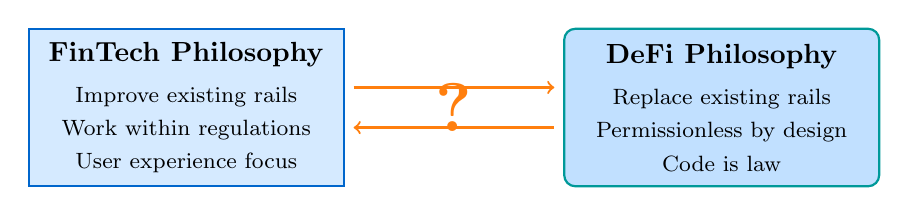
\begin{tikzpicture}[scale=0.85]
% FinTech side
\node[process, minimum width=4cm, minimum height=2cm, align=center] (fintech) at (-4,0) {
\textbf{FinTech Philosophy}\\[3pt]
\footnotesize Improve existing rails\\
\footnotesize Work within regulations\\
\footnotesize User experience focus
};

% DeFi side
\node[blockchain, minimum width=4cm, minimum height=2cm, align=center] (defi) at (4,0) {
\textbf{DeFi Philosophy}\\[3pt]
\footnotesize Replace existing rails\\
\footnotesize Permissionless by design\\
\footnotesize Code is law
};

% Question mark in middle
\node[font=\Huge\bfseries, text=dforange] at (0,0) {?};

% Arrows
\draw[->, thick, dforange] (-1.5,0.3) -- (1.5,0.3);
\draw[<-, thick, dforange] (-1.5,-0.3) -- (1.5,-0.3);
\end{tikzpicture}
\end{center}

\vspace{0.3cm}
\textbf{Key Question:} Are these philosophies incompatible, or are they converging toward common ground?

\begin{itemize}
\item \textbf{2017-2020}: Clear separation---crypto enthusiasts vs. banking innovators
\item \textbf{2021-2024}: Boundaries blur---PayPal adds crypto, Aave adds compliance
\item \textbf{2025+}: Convergence accelerates---hybrid models dominate
\end{itemize}
\end{frame}

% =====================================================================
% SLIDES 5-24: CORE CONTENT
% =====================================================================
\begin{frame}{The Convergence Thesis}
\begin{center}
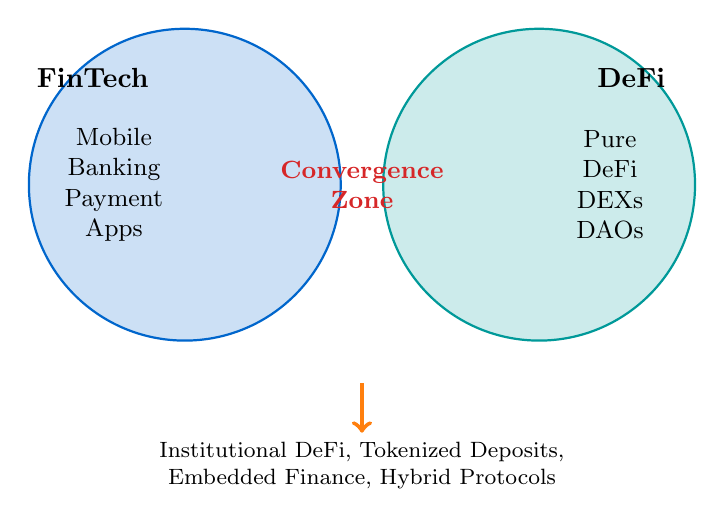
\begin{tikzpicture}[scale=0.9]
% Left circle - FinTech
\draw[thick, dfblue, fill=dfblue!20] (-2.5,0) circle (2.2cm);
\node[font=\bfseries] at (-3.8,1.5) {FinTech};

% Right circle - DeFi
\draw[thick, dfteal, fill=dfteal!20] (2.5,0) circle (2.2cm);
\node[font=\bfseries] at (3.8,1.5) {DeFi};

% Overlap region
\begin{scope}
\clip (-2.5,0) circle (2.2cm);
\fill[dforange!40] (2.5,0) circle (2.2cm);
\end{scope}

% Labels
\node[align=center, font=\small] at (-3.5,0) {Mobile\\Banking\\Payment\\Apps};
\node[align=center, font=\small] at (3.5,0) {Pure\\DeFi\\DEXs\\DAOs};
\node[align=center, font=\small\bfseries, text=dfred] at (0,0) {Convergence\\Zone};

% Arrow below
\draw[->, ultra thick, dforange] (0,-2.8) -- (0,-3.5);
\node[below, font=\footnotesize, align=center] at (0,-3.5) {Institutional DeFi, Tokenized Deposits,\\Embedded Finance, Hybrid Protocols};
\end{tikzpicture}
\end{center}
\end{frame}

\begin{frame}{What Is the Convergence Thesis?}
\begin{block}{Definition}
The \textbf{Convergence Thesis} states that the traditional divide between FinTech (centralized, regulated, institution-based) and DeFi (decentralized, permissionless, code-based) is \textbf{dissolving in practice}.
\end{block}

\vspace{0.3cm}
\textbf{Evidence of Convergence:}
\begin{itemize}
\item FinTech companies adopting crypto features for efficiency and customer demand
\item DeFi protocols adding compliance layers to access institutional capital
\item Traditional banks experimenting with blockchain settlement
\item Hybrid products that blend the best of both worlds
\end{itemize}

\vspace{0.3cm}
\begin{alertblock}{Key Insight}
Convergence is driven by \textbf{pragmatism}---both sides recognize that pure approaches face scalability, adoption, or regulatory barriers.
\end{alertblock}
\end{frame}

\begin{frame}{Why Is Convergence Happening?}
\begin{columns}[T]
\begin{column}{0.48\textwidth}
\textbf{FinTech $\rightarrow$ DeFi:}
\begin{itemize}
\item Cost efficiency (24/7 settlement)
\item Yield opportunities (staking, lending)
\item Programmable money features
\item Customer demand for crypto
\item Competitive pressure
\end{itemize}

\vspace{0.3cm}
\textbf{Examples:}
\begin{itemize}
\item PayPal integrating crypto
\item Robinhood listing tokens
\item Visa settling in USDC
\end{itemize}
\end{column}
\begin{column}{0.48\textwidth}
\textbf{DeFi $\rightarrow$ FinTech:}
\begin{itemize}
\item Regulatory survival
\item Institutional capital access
\item User experience expectations
\item Fiat on/off ramps
\item Compliance requirements
\end{itemize}

\vspace{0.3cm}
\textbf{Examples:}
\begin{itemize}
\item Aave Arc (permissioned pools)
\item Circle (regulated stablecoin)
\item Coinbase (public company, licensed)
\end{itemize}
\end{column}
\end{columns}
\end{frame}

\begin{frame}{Convergence Driver 1: Efficiency Gains}
\begin{block}{The Efficiency Argument}
Blockchain settlement offers measurable improvements over traditional rails:
\end{block}

\begin{center}
\begin{tabular}{lcc}
\toprule
\textbf{Metric} & \textbf{Traditional} & \textbf{Blockchain} \\
\midrule
Settlement time & T+2 days & Minutes to seconds \\
Operating hours & Business hours & 24/7/365 \\
Cross-border cost & 3-7\% & <1\% \\
Intermediaries & 3-5 parties & 0-1 parties \\
Programmability & Limited & Smart contracts \\
\bottomrule
\end{tabular}
\end{center}

\vspace{0.3cm}
\textbf{Why FinTech cares:} Lower costs, better margins, competitive advantage\\
\textbf{Why banks care:} Operational efficiency, reduced counterparty risk
\end{frame}

\begin{frame}{Convergence Driver 2: Regulatory Pressure}
\begin{columns}[T]
\begin{column}{0.48\textwidth}
\textbf{Regulators Pushing Toward Convergence:}
\begin{itemize}
\item MiCA (EU) requires licensing for crypto
\item SEC enforcement against unregistered offerings
\item FATF travel rule for crypto transfers
\item Bank regulators exploring tokenized deposits
\end{itemize}
\end{column}
\begin{column}{0.48\textwidth}
\textbf{Result:}
\begin{itemize}
\item Pure DeFi faces legal challenges
\item Compliant crypto gains legitimacy
\item ``Regulate to innovate'' mindset
\item Hybrid approaches become necessary
\end{itemize}
\end{column}
\end{columns}

\vspace{0.5cm}
\begin{alertblock}{Regulatory Reality}
The choice is increasingly binary: add compliance and survive, or remain pure and face enforcement. Most choose survival.
\end{alertblock}
\end{frame}

\begin{frame}{Convergence Driver 3: Institutional Demand}
\begin{block}{Trillions in Capital Waiting}
Institutional investors want blockchain exposure but require:
\end{block}

\begin{itemize}
\item \textbf{Regulatory clarity}: Clear legal status of assets
\item \textbf{Custody solutions}: Qualified custodians, insurance
\item \textbf{Counterparty verification}: KYC/AML compliance
\item \textbf{Risk management}: Understood, quantifiable risks
\item \textbf{Familiar structures}: Funds, ETFs, regulated vehicles
\end{itemize}

\vspace{0.3cm}
\textbf{Institutional DeFi emerges to serve this demand:}
\begin{itemize}
\item Same smart contracts, restricted access
\item Whitelisted wallet addresses
\item Compliance layer on-chain or off-chain
\end{itemize}
\end{frame}

\begin{frame}{Convergence Example 1: Institutional DeFi}
\begin{block}{Definition}
DeFi protocols or pools designed for institutions with KYC/AML, permissioned access, and regulatory compliance.
\end{block}

\begin{columns}[T]
\begin{column}{0.48\textwidth}
\textbf{How it works:}
\begin{itemize}
\item Whitelisted wallet addresses
\item Identity verification required
\item Compliance layer on-chain or off-chain
\item Same smart contracts, restricted access
\end{itemize}
\end{column}
\begin{column}{0.48\textwidth}
\textbf{Key examples:}
\begin{itemize}
\item \textbf{Aave Arc}: Permissioned Aave for institutions
\item \textbf{Compound Treasury}: Institutional lending product
\item \textbf{Maple Finance}: Institutional credit pools
\item \textbf{Centrifuge}: Real-world asset financing
\end{itemize}
\end{column}
\end{columns}

\vspace{0.3cm}
\begin{alertblock}{Key Insight}
Same DeFi rails, different access model. The technology does not change; the \emph{governance layer} does.
\end{alertblock}
\end{frame}

\begin{frame}{Deep Dive: How Aave Arc Works}
\begin{center}
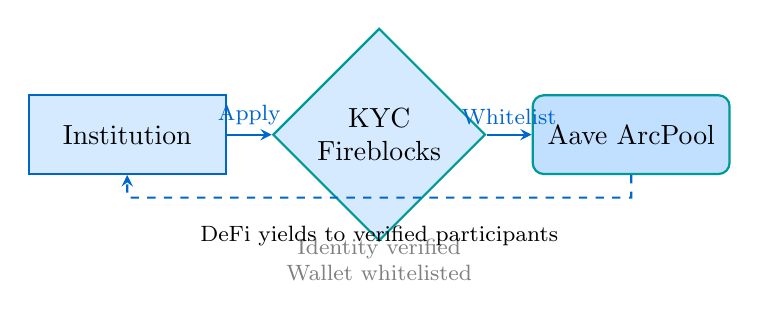
\begin{tikzpicture}[scale=0.8]
% Institution
\node[process, minimum width=2.5cm] (inst) at (-4,0) {Institution};

% KYC Layer
\node[decision, minimum width=2cm, minimum height=1.5cm, align=center] (kyc) at (0,0) {KYC\\Fireblocks};

% Aave Arc Pool
\node[blockchain, minimum width=2.5cm] (pool) at (4,0) {Aave Arc\\Pool};

% Arrows
\draw[arrow] (inst) -- node[above, font=\footnotesize] {Apply} (kyc);
\draw[arrow] (kyc) -- node[above, font=\footnotesize] {Whitelist} (pool);

% Verification flow
\node[below, font=\footnotesize, text=dfgray, align=center] at (0,-1.5) {Identity verified\\Wallet whitelisted};

% Returns (dashed arrow back)
\draw[thick, dashed, ->, >=stealth, color=dfblue] (pool.south) -- (4,-1) -- (-4,-1) -- (inst.south);
\node[below, font=\footnotesize] at (0,-1.3) {DeFi yields to verified participants};
\end{tikzpicture}
\end{center}

\vspace{0.3cm}
\textbf{Key Features:}
\begin{itemize}
\item Fireblocks provides identity verification and custody
\item Only whitelisted addresses can interact with Arc pools
\item Smart contracts identical to permissionless Aave
\item Institutions get DeFi yields with compliance
\end{itemize}
\end{frame}

\begin{frame}{Convergence Example 2: Tokenized Deposits}
\begin{block}{Definition}
Bank deposits represented as tokens on a blockchain, combining bank liability with blockchain programmability.
\end{block}

\begin{center}
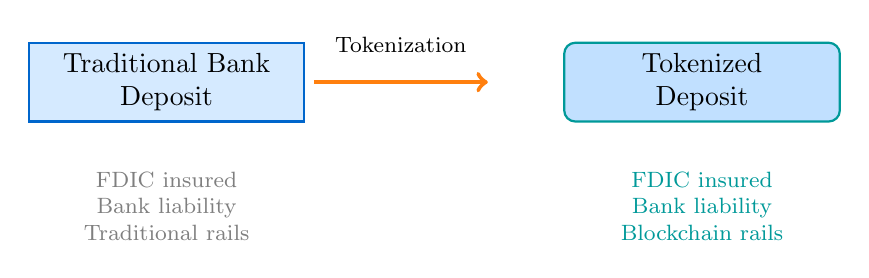
\begin{tikzpicture}[scale=0.85]
% Traditional deposit
\node[process, minimum width=3.5cm, align=center] (bank) at (-4,0) {Traditional Bank\\Deposit};

% Arrow
\draw[->, ultra thick, dforange] (-1.8,0) -- (0.8,0);
\node[above, font=\footnotesize] at (-0.5,0.3) {Tokenization};

% Tokenized deposit
\node[blockchain, minimum width=3.5cm, align=center] (token) at (4,0) {Tokenized\\Deposit};

% Properties below
\node[below, font=\footnotesize, align=center, text=dfgray] at (-4,-1.2) {FDIC insured\\Bank liability\\Traditional rails};
\node[below, font=\footnotesize, align=center, text=dfteal] at (4,-1.2) {FDIC insured\\Bank liability\\Blockchain rails};
\end{tikzpicture}
\end{center}

\textbf{Key players:} JPMorgan (JPM Coin), Citi, Wells Fargo, Societe Generale

\textbf{Difference from stablecoins:} Tokenized deposits are \emph{bank liabilities}, not claims on reserves held by a separate issuer.
\end{frame}

\begin{frame}{Tokenized Deposits vs. Stablecoins}
\begin{center}
\begin{tabular}{lcc}
\toprule
\textbf{Feature} & \textbf{Tokenized Deposit} & \textbf{Stablecoin (e.g., USDC)} \\
\midrule
Liability type & Bank liability & Issuer liability \\
Deposit insurance & Yes (if applicable) & No \\
Issuer & Commercial bank & Crypto company \\
Backing & Bank balance sheet & Reserve assets \\
Regulation & Banking regulation & Varies by jurisdiction \\
Redemption & Direct with bank & Through issuer \\
\bottomrule
\end{tabular}
\end{center}

\vspace{0.3cm}
\begin{exampleblock}{Why It Matters}
Tokenized deposits bring \textbf{banking-grade safety} (deposit insurance, bank oversight) to blockchain rails. This could enable institutional adoption at scale.
\end{exampleblock}
\end{frame}

\begin{frame}{Convergence Example 3: Embedded Finance}
\begin{block}{Definition}
Financial services seamlessly integrated into non-financial platforms and workflows.
\end{block}

\begin{columns}[T]
\begin{column}{0.55\textwidth}
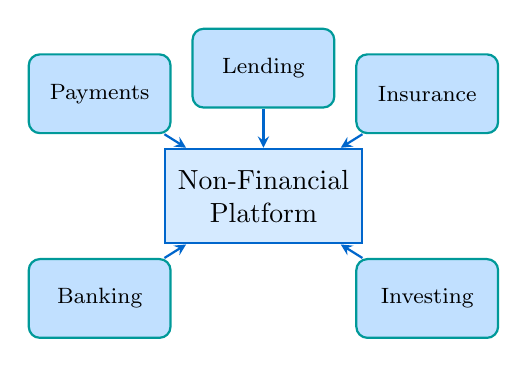
\begin{tikzpicture}[scale=0.65]
% Central platform
\node[process, minimum width=2.5cm, minimum height=1.2cm, align=center] (platform) at (0,0) {Non-Financial\\Platform};

% Surrounding services
\node[blockchain, minimum width=1.8cm, font=\footnotesize] (pay) at (-3.2,2) {Payments};
\node[blockchain, minimum width=1.8cm, font=\footnotesize] (lend) at (0,2.5) {Lending};
\node[blockchain, minimum width=1.8cm, font=\footnotesize] (ins) at (3.2,2) {Insurance};
\node[blockchain, minimum width=1.8cm, font=\footnotesize] (inv) at (3.2,-2) {Investing};
\node[blockchain, minimum width=1.8cm, font=\footnotesize] (bank) at (-3.2,-2) {Banking};

% Arrows
\draw[arrow] (pay) -- (platform);
\draw[arrow] (lend) -- (platform);
\draw[arrow] (ins) -- (platform);
\draw[arrow] (inv) -- (platform);
\draw[arrow] (bank) -- (platform);
\end{tikzpicture}
\end{column}
\begin{column}{0.42\textwidth}
\textbf{Examples:}
\begin{itemize}
\item Shopify Capital (e-commerce lending)
\item Uber driver instant pay
\item Apple Pay Later
\item Amazon lending to sellers
\item Tesla insurance
\end{itemize}

\vspace{0.3cm}
\textbf{Crypto angle:}
\begin{itemize}
\item Crypto payouts in apps
\item DeFi yields embedded in wallets
\item NFT financing at checkout
\end{itemize}
\end{column}
\end{columns}
\end{frame}

\begin{frame}{Embedded Finance: The Convergence Catalyst}
\textbf{Why Embedded Finance Accelerates Convergence:}

\begin{enumerate}
\item \textbf{Invisible infrastructure}: Users do not see ``DeFi'' or ``FinTech''---just seamless service
\item \textbf{Best tool for the job}: Platforms choose blockchain or traditional rails based on efficiency
\item \textbf{API-driven}: Both DeFi protocols and banks offer API access
\item \textbf{User experience trumps ideology}: What works, wins
\end{enumerate}

\vspace{0.3cm}
\begin{exampleblock}{Example: Shopify + Crypto}
Shopify integrates:
\begin{itemize}
\item Traditional payment processing (Stripe)
\item Cryptocurrency payments (BitPay)
\item Seller financing (Shopify Capital)
\item Potential: DeFi lending pools for merchant financing
\end{itemize}
The merchant sees one platform; underneath, multiple financial rails.
\end{exampleblock}
\end{frame}

\begin{frame}{Convergence Example 4: Hybrid Protocols}
\begin{columns}[T]
\begin{column}{0.48\textwidth}
\textbf{What makes them hybrid?}
\begin{itemize}
\item On-chain execution + off-chain compliance
\item Decentralized protocol + centralized governance
\item Crypto assets + real-world assets
\item Permissionless base + permissioned layers
\end{itemize}
\end{column}
\begin{column}{0.48\textwidth}
\textbf{Examples:}
\begin{itemize}
\item \textbf{MakerDAO}: DAI backed by RWA vaults
\item \textbf{Ondo Finance}: Tokenized treasuries
\item \textbf{Backed Finance}: Tokenized ETFs
\item \textbf{Goldfinch}: Credit to emerging markets
\end{itemize}
\end{column}
\end{columns}

\vspace{0.5cm}
\begin{exampleblock}{MakerDAO's RWA Strategy}
MakerDAO now allocates \$2B+ to real-world assets (US Treasuries, corporate bonds). A ``DeFi'' protocol holding TradFi assets---convergence in action.
\end{exampleblock}
\end{frame}

\begin{frame}{Deep Dive: MakerDAO's Real-World Assets}
\begin{center}
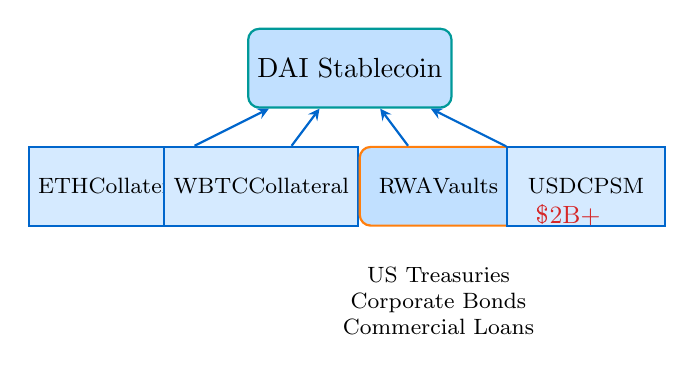
\begin{tikzpicture}[scale=0.75]
% DAI
\node[blockchain, minimum width=2.5cm] (dai) at (0,2) {DAI Stablecoin};

% Collateral types
\node[process, minimum width=2cm, font=\footnotesize] (eth) at (-4,0) {ETH\\Collateral};
\node[process, minimum width=2cm, font=\footnotesize] (btc) at (-1.5,0) {WBTC\\Collateral};
\node[aibox, minimum width=2cm, font=\footnotesize] (rwa) at (1.5,0) {RWA\\Vaults};
\node[process, minimum width=2cm, font=\footnotesize] (usdc) at (4,0) {USDC\\PSM};

% Arrows
\draw[arrow] (eth) -- (dai);
\draw[arrow] (btc) -- (dai);
\draw[arrow] (rwa) -- (dai);
\draw[arrow] (usdc) -- (dai);

% RWA breakdown
\node[below, font=\footnotesize, align=center] at (1.5,-1.2) {US Treasuries\\Corporate Bonds\\Commercial Loans};

% Percentage
\node[right, font=\small, text=dfred] at (3,-0.5) {\$2B+};
\end{tikzpicture}
\end{center}

\textbf{Implications:}
\begin{itemize}
\item DeFi protocol now depends on TradFi counterparties
\item Diversifies collateral risk beyond crypto volatility
\item Requires trust in off-chain asset custodians
\item Blurs the line between DeFi and traditional finance
\end{itemize}
\end{frame}

\begin{frame}{Visa Settling in USDC: A Milestone}
\begin{block}{What Happened}
In 2021, Visa began settling transactions with partners using USDC stablecoin on Ethereum, later expanding to Solana.
\end{block}

\textbf{Why This Matters:}
\begin{enumerate}
\item \textbf{Validation}: World's largest payment network using crypto rails
\item \textbf{Efficiency}: 24/7 settlement, reduced counterparty risk
\item \textbf{Programmability}: Smart contract-enabled payments
\item \textbf{Hybrid model}: Traditional Visa network + blockchain settlement
\end{enumerate}

\vspace{0.3cm}
\begin{alertblock}{Convergence in Action}
Visa did not become a ``crypto company.'' It integrated blockchain where it made business sense while maintaining its core regulated infrastructure.
\end{alertblock}
\end{frame}

\begin{frame}{Hybrid Custody: Blending Self-Custody and Institutional}
\begin{columns}[T]
\begin{column}{0.48\textwidth}
\textbf{Pure Self-Custody:}
\begin{itemize}
\item User controls private keys
\item No recovery if keys lost
\item Maximum sovereignty
\item Requires technical knowledge
\end{itemize}
\end{column}
\begin{column}{0.48\textwidth}
\textbf{Pure Institutional Custody:}
\begin{itemize}
\item Institution holds keys
\item Recovery possible
\item Counterparty risk
\item Familiar to traditional users
\end{itemize}
\end{column}
\end{columns}

\vspace{0.3cm}
\begin{block}{Hybrid Custody Solutions}
\begin{itemize}
\item \textbf{Multi-sig wallets}: 2-of-3 keys (user, institution, backup)
\item \textbf{Social recovery}: Designated guardians can restore access
\item \textbf{Tiered access}: Small amounts self-custody, large amounts require verification
\item \textbf{MPC (Multi-Party Computation)}: Key shares distributed, no single point of failure
\end{itemize}
\end{block}
\end{frame}

\begin{frame}{Which Innovations Cross the Divide?}
\begin{center}
\textbf{Framework for Evaluating Convergence Likelihood}
\end{center}

\begin{table}[h]
\centering
\small
\begin{tabular}{lcc}
\toprule
\textbf{Factor} & \textbf{High Likelihood} & \textbf{Low Likelihood} \\
\midrule
Regulatory clarity & Clear path & Fundamental conflict \\
Institutional demand & Strong & Weak/retail-only \\
User experience & Comparable to TradFi & Significantly worse \\
Risk profile & Understood, manageable & Novel, unquantifiable \\
Value proposition & Clear efficiency gain & Ideological appeal only \\
\bottomrule
\end{tabular}
\end{table}

\vspace{0.3cm}
\textbf{Most likely to converge:} Payments, lending, asset tokenization\\
\textbf{Least likely:} Privacy coins, fully anonymous DeFi, unregistered securities
\end{frame}

\begin{frame}{Technology Stack Blending}
\begin{block}{Definition}
Architectures that strategically combine traditional infrastructure with blockchain layers for optimal efficiency.
\end{block}

\textbf{Examples:}
\begin{itemize}
\item \textbf{Hybrid databases}: Traditional DB for non-critical data, blockchain for settlement
\item \textbf{Layer 2 solutions}: Centralized sequencers, decentralized verification
\item \textbf{Private + Public chains}: Internal private blockchain, public chain for finality
\item \textbf{API gateways}: Centralized access to decentralized protocols
\end{itemize}

\vspace{0.3cm}
\begin{alertblock}{Design Principle}
Not everything needs to be on-chain. Optimal systems blend technologies based on what each does best.
\end{alertblock}
\end{frame}

\begin{frame}{Cross-Chain Interoperability: The Connector}
\textbf{Why Interoperability Matters for Convergence:}
\begin{itemize}
\item Enables value transfer between different blockchains
\item Connects blockchain and traditional systems
\item Breaks down liquidity silos
\item Improves user experience (no manual bridging)
\end{itemize}

\vspace{0.3cm}
\textbf{Solutions:}
\begin{itemize}
\item \textbf{Bridges}: Cross-chain asset transfers (security challenges)
\item \textbf{Chain abstraction}: Hide chain complexity from users
\item \textbf{Standardized protocols}: Common messaging formats
\item \textbf{SWIFT integration}: Traditional banking meeting blockchain
\end{itemize}

\vspace{0.3cm}
\begin{exampleblock}{SWIFT + Chainlink}
SWIFT (traditional interbank messaging) partnered with Chainlink to enable blockchain interoperability---a direct FinTech-DeFi bridge.
\end{exampleblock}
\end{frame}

\begin{frame}{Barriers to Convergence}
\textbf{What Slows Convergence Down?}

\begin{columns}[T]
\begin{column}{0.48\textwidth}
\textbf{Technical Barriers:}
\begin{itemize}
\item Legacy system integration complexity
\item Blockchain scalability limits
\item Security risks (bridge vulnerabilities)
\item Interoperability challenges
\end{itemize}
\end{column}
\begin{column}{0.48\textwidth}
\textbf{Non-Technical Barriers:}
\begin{itemize}
\item Regulatory uncertainty
\item Cultural resistance (both sides)
\item Conflicting incentives
\item Talent shortage
\end{itemize}
\end{column}
\end{columns}

\vspace{0.3cm}
\begin{alertblock}{Overcoming Barriers Requires:}
\begin{itemize}
\item Time and regulatory evolution
\item Successful case studies demonstrating value
\item Technical maturation of blockchain infrastructure
\item Aligned incentives across stakeholder groups
\end{itemize}
\end{alertblock}
\end{frame}

% =====================================================================
% SLIDES 25-28: ADDITIONAL CONTENT (CASE STUDIES)
% =====================================================================
\begin{frame}{Case Study 1: BlackRock's BUIDL Fund}
\begin{block}{Background}
In 2024, BlackRock (world's largest asset manager, \$10T+ AUM) launched BUIDL---a tokenized fund for US Treasury exposure on Ethereum.
\end{block}

\textbf{Key Features:}
\begin{itemize}
\item Tokenized shares representing US Treasury holdings
\item 24/7 transferability on blockchain
\item Institutional-grade compliance (KYC required)
\item Integration with DeFi protocols as collateral
\end{itemize}

\vspace{0.3cm}
\textbf{Convergence Significance:}
\begin{itemize}
\item TradFi giant embracing blockchain infrastructure
\item ``Safe'' asset (Treasuries) in DeFi ecosystem
\item Signals institutional acceptance of tokenization
\end{itemize}
\end{frame}

\begin{frame}{Case Study 2: Singapore's Project Guardian}
\begin{block}{Background}
Project Guardian is a collaborative initiative by the Monetary Authority of Singapore (MAS) with major banks to test asset tokenization.
\end{block}

\textbf{Participants:} DBS Bank, JPMorgan, Standard Chartered, HSBC, and others

\textbf{Tested Use Cases:}
\begin{itemize}
\item Tokenized bonds trading and settlement
\item Foreign exchange transactions on blockchain
\item Asset-backed securities tokenization
\item Cross-border payments
\end{itemize}

\vspace{0.3cm}
\textbf{Key Finding:} Tokenization can improve efficiency by 30-50\% in trade settlement while maintaining regulatory compliance.
\end{frame}

\begin{frame}{Case Study 3: Coinbase---From Exchange to Financial Institution}
\begin{columns}[T]
\begin{column}{0.48\textwidth}
\textbf{Coinbase's Evolution:}
\begin{itemize}
\item 2012: Bitcoin exchange
\item 2018: Custody for institutions
\item 2021: Public company (NASDAQ)
\item 2023: Licensed in multiple jurisdictions
\item 2024: Banking partnerships, Base L2
\end{itemize}
\end{column}
\begin{column}{0.48\textwidth}
\textbf{Convergence Features:}
\begin{itemize}
\item SEC-regulated entity
\item Institutional custody (Coinbase Prime)
\item Fiat banking integration
\item Layer 2 blockchain (Base)
\item Stablecoin partnership (USDC)
\end{itemize}
\end{column}
\end{columns}

\vspace{0.3cm}
\begin{alertblock}{The Transformation}
Coinbase demonstrates how a crypto-native company becomes a regulated financial institution while maintaining blockchain infrastructure.
\end{alertblock}
\end{frame}

\begin{frame}{Case Study 4: Circle and USDC---The Compliant Stablecoin}
\begin{block}{Circle's Strategy}
Build a ``digital dollar'' that is fully compliant, transparent, and integrated with traditional finance.
\end{block}

\textbf{Compliance Features:}
\begin{itemize}
\item Monthly attestations by Grant Thornton
\item US state money transmitter licenses
\item Reserves in US Treasuries and cash
\item Partnerships with major banks (BNY Mellon)
\end{itemize}

\textbf{Integration with TradFi:}
\begin{itemize}
\item Visa settlement partnership
\item Mastercard integration
\item Apple Pay compatibility
\item Cross-border remittances
\end{itemize}

\textbf{Result:} USDC is accepted by both DeFi protocols AND traditional financial institutions.
\end{frame}

% =====================================================================
% SLIDES 29-30: DISCUSSION/APPLICATION
% =====================================================================
\begin{frame}{Discussion: The Convergence Trade-offs}
\begin{columns}[T]
\begin{column}{0.48\textwidth}
\begin{alertblock}{What Is Lost in Convergence?}
\begin{itemize}
\item Permissionlessness
\item Censorship resistance
\item Privacy/pseudonymity
\item Trustlessness
\item Decentralization purity
\end{itemize}
\end{alertblock}
\end{column}
\begin{column}{0.48\textwidth}
\begin{exampleblock}{What Is Gained?}
\begin{itemize}
\item Regulatory acceptance
\item Institutional capital
\item Consumer protection
\item Mainstream adoption
\item Integration with existing systems
\end{itemize}
\end{exampleblock}
\end{column}
\end{columns}

\vspace{0.5cm}
\begin{block}{Discussion Questions}
\begin{enumerate}
\item Is ``permissioned DeFi'' still DeFi?
\item Will the permissionless layer survive alongside the permissioned one?
\item Who benefits most from convergence?
\end{enumerate}
\end{block}
\end{frame}

\begin{frame}{Application: Analyzing a Convergence Opportunity}
\begin{block}{Framework Application}
For a proposed convergence initiative, evaluate:
\end{block}

\begin{enumerate}
\item \textbf{Regulatory clarity}: Is there a clear legal path?
\item \textbf{Institutional demand}: Do institutions actually want this?
\item \textbf{User experience}: Can mainstream users understand it?
\item \textbf{Risk profile}: Are the risks quantifiable?
\item \textbf{Value proposition}: What is the clear efficiency gain?
\end{enumerate}

\vspace{0.3cm}
\textbf{Exercise: Apply this framework to:}
\begin{itemize}
\item Tokenized real estate
\item Decentralized identity for banking
\item Algorithmic stablecoins
\item NFTs as collateral for loans
\end{itemize}

Which has the highest convergence likelihood? Why?
\end{frame}

% =====================================================================
% SLIDE 31: EXECUTIVE SUMMARY
% =====================================================================
\begin{frame}{Executive Summary: The Convergence Thesis}
\begin{block}{Key Takeaways}
\begin{enumerate}
\item \textbf{Convergence is real}: The FinTech/DeFi divide is dissolving as each adopts features from the other
\item \textbf{Drivers are pragmatic}: Efficiency, regulation, institutional demand, and user experience push convergence
\item \textbf{Hybrid models dominate}: Institutional DeFi, tokenized deposits, embedded finance, and hybrid protocols represent the future
\item \textbf{Trade-offs exist}: Convergence sacrifices some crypto-native properties (permissionlessness, privacy) for mainstream adoption
\item \textbf{Framework matters}: Regulatory clarity, institutional demand, UX, risk profile, and value proposition determine convergence likelihood
\end{enumerate}
\end{block}

\vspace{0.3cm}
\begin{alertblock}{Bottom Line}
The future of finance is neither purely centralized nor purely decentralized---it is \textbf{hybrid}, blending the best of both worlds.
\end{alertblock}
\end{frame}

% =====================================================================
% SLIDE 32: CONCEPT MAP
% =====================================================================
\begin{frame}{Concept Map: The Convergence Landscape}
\begin{center}
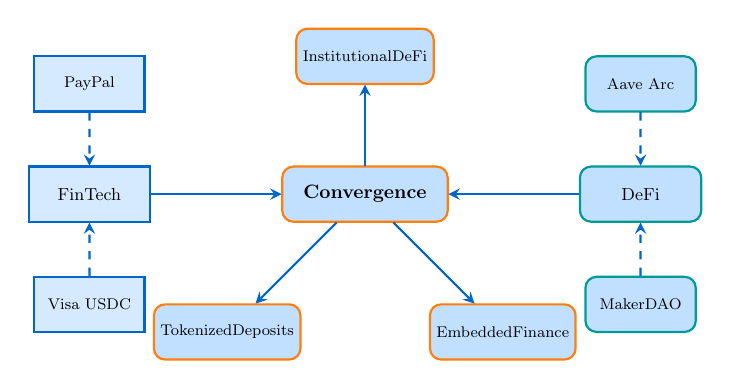
\begin{tikzpicture}[scale=0.7, transform shape]
% Central node
\node[aibox, minimum width=3cm, font=\bfseries] (conv) at (0,0) {Convergence};

% FinTech side
\node[process, minimum width=2.2cm, font=\small] (fintech) at (-5,0) {FinTech};
\node[process, minimum width=2cm, font=\footnotesize] (paypal) at (-5,2) {PayPal};
\node[process, minimum width=2cm, font=\footnotesize] (visa) at (-5,-2) {Visa USDC};

% DeFi side
\node[blockchain, minimum width=2.2cm, font=\small] (defi) at (5,0) {DeFi};
\node[blockchain, minimum width=2cm, font=\footnotesize] (aave) at (5,2) {Aave Arc};
\node[blockchain, minimum width=2cm, font=\footnotesize] (maker) at (5,-2) {MakerDAO};

% Convergence examples
\node[aibox, minimum width=2cm, font=\footnotesize] (inst) at (0,2.5) {Institutional\\DeFi};
\node[aibox, minimum width=2cm, font=\footnotesize] (token) at (-2.5,-2.5) {Tokenized\\Deposits};
\node[aibox, minimum width=2cm, font=\footnotesize] (embed) at (2.5,-2.5) {Embedded\\Finance};

% Arrows
\draw[arrow] (fintech) -- (conv);
\draw[arrow] (defi) -- (conv);
\draw[arrow] (conv) -- (inst);
\draw[arrow] (conv) -- (token);
\draw[arrow] (conv) -- (embed);
\draw[arrow, dashed] (paypal) -- (fintech);
\draw[arrow, dashed] (visa) -- (fintech);
\draw[arrow, dashed] (aave) -- (defi);
\draw[arrow, dashed] (maker) -- (defi);
\end{tikzpicture}
\end{center}
\end{frame}

% =====================================================================
% SLIDES 33-34: KEY TERMS
% =====================================================================
\begin{frame}{Key Terms (1/2)}
\begin{description}
\item[Convergence Thesis] The idea that FinTech and DeFi are adopting each other's features, dissolving the traditional divide
\item[Institutional DeFi] DeFi protocols with KYC/AML, permissioned access, designed for institutional participants
\item[Tokenized Deposits] Bank deposits represented as blockchain tokens, maintaining bank liability status
\item[Embedded Finance] Financial services integrated seamlessly into non-financial platforms
\item[Hybrid Protocol] Systems combining on-chain execution with off-chain compliance or real-world assets
\item[Permissioned DeFi] DeFi protocols that restrict access to verified participants
\end{description}
\end{frame}

\begin{frame}{Key Terms (2/2)}
\begin{description}
\item[Real-World Assets (RWA)] Traditional financial assets (bonds, loans, real estate) tokenized on blockchain
\item[Hybrid Custody] Custody solutions blending self-custody with institutional safeguards
\item[Technology Stack Blending] Architectures combining traditional and blockchain infrastructure
\item[Compliance-Friendly DeFi] Protocols designed with regulatory requirements from inception
\item[Cross-Chain Interoperability] Ability to transfer value and data between different blockchains
\item[Chain Abstraction] Hiding blockchain complexity from end users
\end{description}
\end{frame}

% =====================================================================
% SLIDE 35: COMMON MISCONCEPTIONS
% =====================================================================
\begin{frame}{Common Misconceptions}
\begin{alertblock}{Misconception 1: ``Convergence means DeFi is dead''}
\textbf{Reality:} Permissionless DeFi will likely coexist with permissioned versions. Different use cases require different access models.
\end{alertblock}

\begin{alertblock}{Misconception 2: ``All FinTech will move to blockchain''}
\textbf{Reality:} Blockchain adoption is selective. Traditional rails remain superior for many use cases. Convergence is about adding options, not replacing everything.
\end{alertblock}

\begin{alertblock}{Misconception 3: ``Tokenized deposits = stablecoins''}
\textbf{Reality:} Critical difference---tokenized deposits are direct bank liabilities with deposit insurance; stablecoins are claims on separate issuers.
\end{alertblock}

\begin{alertblock}{Misconception 4: ``Compliance kills innovation''}
\textbf{Reality:} Compliance enables institutional capital and mainstream adoption, which can fund more innovation.
\end{alertblock}
\end{frame}

% =====================================================================
% SLIDES 36-37: SELF-ASSESSMENT QUESTIONS
% =====================================================================
\begin{frame}{Self-Assessment Questions (1/2)}
\begin{block}{Question 1}
What is the fundamental concept of the Convergence Thesis?
\begin{enumerate}[A.]
\item All cryptocurrencies will eventually merge into a single blockchain
\item The traditional divide between FinTech and DeFi is dissolving as both adopt features from the other
\item Banks will completely replace blockchain technology
\item Cryptocurrency will become illegal worldwide
\end{enumerate}
\end{block}
\vspace{0.2cm}
\textit{Answer: B. The Convergence Thesis describes how FinTech and DeFi are adopting each other's features---FinTech adopts crypto for efficiency, DeFi adds compliance for institutional access.}
\end{frame}

\begin{frame}{Self-Assessment Questions (2/2)}
\begin{block}{Question 2}
Visa's strategy of settling transactions in USDC stablecoin represents:
\begin{enumerate}[A.]
\item Visa abandoning traditional payment rails entirely
\item A convergence move where a traditional payment network integrates blockchain for settlement efficiency
\item A marketing gimmick with no practical implementation
\item Visa becoming a cryptocurrency exchange
\end{enumerate}
\end{block}
\textit{Answer: B. Visa remains a traditional, regulated network but integrated blockchain settlement for efficiency.}

\vspace{0.3cm}
\begin{block}{Question 3}
What are the primary trade-offs LOST in the convergence process?
\begin{enumerate}[A.]
\item Transaction speed and security
\item Permissionlessness, censorship resistance, privacy, trustlessness
\item User interface quality and customer support
\item Profitability and market share
\end{enumerate}
\end{block}
\textit{Answer: B. Convergence sacrifices key crypto-native properties for mainstream adoption.}
\end{frame}

% =====================================================================
% SLIDE 38: WHAT'S NEXT
% =====================================================================
\begin{frame}{What's Next: Topic 6.2 -- AI and Digital Finance}
\begin{columns}[T]
\begin{column}{0.48\textwidth}
\textbf{Coming Up:}
\begin{itemize}
\item AI applications in finance
\item Machine learning for risk management
\item Algorithmic trading strategies
\item AI + blockchain convergence
\item Regulatory implications of AI in finance
\end{itemize}
\end{column}
\begin{column}{0.48\textwidth}
\textbf{Connection to Convergence:}
\begin{itemize}
\item AI enables smarter hybrid systems
\item Automated compliance (RegTech)
\item AI-driven risk assessment for DeFi
\item Natural language interfaces
\item Predictive analytics for both FinTech and DeFi
\end{itemize}
\end{column}
\end{columns}

\vspace{0.5cm}
\begin{block}{Preview Question}
How might AI accelerate or change the convergence between FinTech and DeFi? Consider both opportunities and risks.
\end{block}
\end{frame}

% =====================================================================
% SLIDE 39: RESOURCES
% =====================================================================
\begin{frame}{Resources for Further Study}
\textbf{Academic Papers:}
\begin{itemize}
\item ``Tokenization of Financial Assets'' -- Bank for International Settlements
\item ``DeFi: Decentralized Finance'' -- Federal Reserve Bank of St. Louis
\end{itemize}

\textbf{Industry Reports:}
\begin{itemize}
\item Project Guardian reports (Monetary Authority of Singapore)
\item Chainalysis ``State of Crypto'' annual reports
\item World Economic Forum blockchain reports
\end{itemize}

\textbf{Websites and Tools:}
\begin{itemize}
\item DeFi Llama (defilama.com) -- DeFi protocol tracking
\item The Block Research -- Industry analysis
\item CoinDesk -- News and analysis
\end{itemize}

\textbf{Course Materials:}
\begin{itemize}
\item Review Day 1-5 materials for foundational concepts
\item Quiz 6.1 for self-assessment
\end{itemize}
\end{frame}

% =====================================================================
% SLIDE 40: QUESTIONS?
% =====================================================================
\begin{frame}
\begin{center}
\vspace{2cm}
{\Huge \textbf{Questions?}}

\vspace{1.5cm}
{\large Topic 6.1: The Convergence Thesis}

\vspace{0.5cm}
{\normalsize FinTech and DeFi Coming Together}

\vspace{1.5cm}
\textcolor{dfgray}{Digital Finance | Joerg Osterrieder | 2025}
\end{center}
\end{frame}

\end{document}
